\chapterimage{ChapterImages/Requirements}
\chapter{Design Specifications}
%\chapter{Design Description}   %This title will make more sense in Winter and Spring.
\label{design-description}

%%%%%%%%%%%%%%%%
% \begin{remark}\color{blue}
% This \textbf{Design Description} chapter defines what the design is. For fall, it's really your vision or proposal for what you think the design might be by the end of winter or spring quarter. So let's call it the \textbf{Design Vision} in the fall documents. It will be a short chapter. 
% Even so, on the basis of preliminary need-finding, benchmarking and critical function evaluation, you have some idea of what may be appropriate. \emph{Take a point of view and assert it!}  
% \begin{itemize}
% \item A CAD rendering or systems diagram, or schematic, or a concept drawing is appropriate to help explain your vision. 
% \item If you find yourself adding rationale, or discussing design alternatives or how the vision came about, you are writing text that should be moved into the end of the Development section. This is section is about what the design (or vision) is, not how it came to be.
% \end{itemize}
% \normalcolor \end{remark}
%%%%%%%%%%%%%%%%


%\section{Vision}
%\label{vision}
%
%For winter, although you now have a design to describe, you probably want to start off your Design Description chapter with a reminder of the overall vision, toward which your current design is an important intermediate step.
%
%Use this section to describe your vision or proposal for what you think the design might be. Ideally you should have a sketch, a diagram or other images to help define it.  
%\section{Specifications}
%\label{specifications}
%
%In winter and spring here is where you describe what your design is. 
%\begin{itemize}
%\item Define the subsystems and how they go together.
%\item Use diagrams, CAD renderings, tables, etc. to make it clear. 
%\item Use flow charts or pseudocode to describe procedures.
%\item Detailed source code and numerical data should go in an Appendix section or, if really long, on a CD or other electronic format (nobody will wade through the printout).
%\end{itemize}
\vspace{1em}

Several prototypes were built to explore how we might improve the simplicity of interfacing with smart home technology, and how we might improve the transition between home and car. We capitalized on the need for users to (1) enjoy peace of mind about their home and car at all times, given that security is the primary reason users adopt smart home technology, (2) remember important items in their daily routine.
\section{Critical Experience Prototype: Leave-home Button}

For a long time, we have talked about some sort of physical system that is in the house that conveys information about the car and journey ahead to the driver as they are getting ready to leave. We wanted to see what information would be useful to people, and if they would be able to listening to it as they are busy getting ready. So for the critical experience prototype, Stanford team decided to a simple interactive button using the RBBB that the user would press as they are leaving home. This button triggers smart home conditional statements (e.g. turn off lights and lock door behind you) and conveys information about the car and trip ahead (e.g. sending navigation to car, turning on heat). The audio feedback tells users that their command was detected. Useful information would be pushed to user’s phone and car as desired.

We wanted the users to have some kind of distracting activity, mimicking picking up and finding things before they leave the house. People report they are often looking for their wallet, brushing their teeth, etc. So we designed a card sorting task in our experiment to mimic that process.

\begin{figure}
\centering
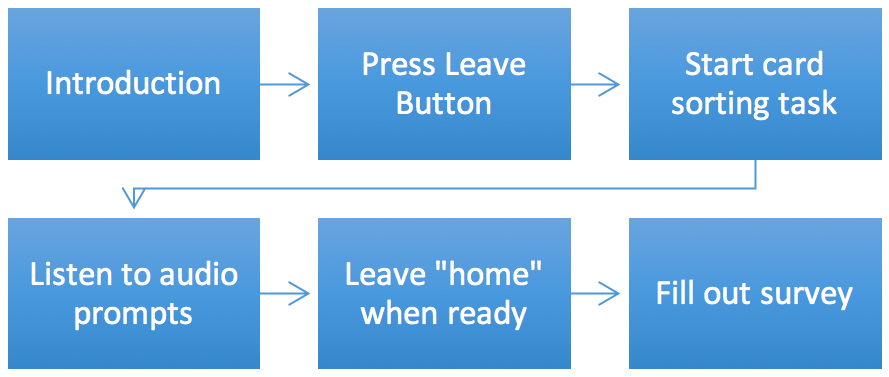
\includegraphics[width=5in]{Figures/Prototypes/CEP/CEPprocedure.png}
	\caption{CEP user testing procedure}
		\label{fig:CEPprocedure}
\end{figure}

The insights we got from user testing are: 1. Rated usefulness of information was mixed, but almost everyone found it helpful to preheat car or adjust temperature before leaving home. Information should be customizable – not everything needs to be said every day. But there is potential value in this information; 2. Exact action suggestion would be more useful than telling information about temperature or car status, for example, Some people did bring umbrella as suggested; 3. The most frequent thing to do before leaving home is to check keys \&{} the most frequent thing to do after arriving home is to turn on the light and take off shoes. So we could look at what people do when they sit in car.

\begin{figure}
\centering
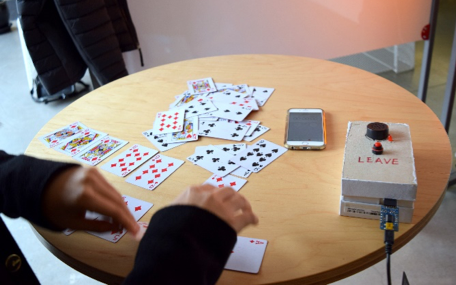
\includegraphics[width=5in]{Figures/Prototypes/CEP/CEPtest1.png}
	\caption{CEP user testing}
		\label{fig:CEPtest1}
\end{figure}

\begin{figure}
\centering
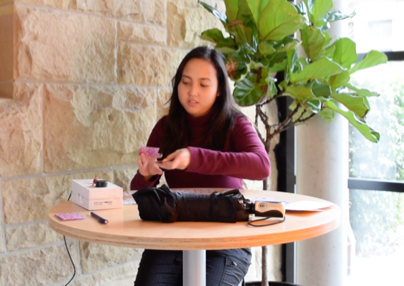
\includegraphics[width=5in]{Figures/Prototypes/CEP/CEPtest2.png}
	\caption{CEP user testing}
		\label{fig:CEPtest2}
\end{figure}

Other insights in terms of improving for future work are:

\begin{itemize}
    \item We could do a better job of setting up the scenario – some people were confused. 
    \item One person wanted a more interactive experience – the system would respond to their voice (could be done with Amazon Echo).
    \item Difficulty: we need to simulate a series of experiences in a whole environment rather than a single one. 
    \item Limitations of map: People were confused about the map’s route to their car. The route should rotate to match the exit’s direction; some descriptive information would also be helpful. If the map was pushed to phone, this would be more useful.
    \item Incorporate security element (e.g. car alerts authorities if you don’t show up after a certain amount of time)
\end{itemize}


\section{Dark Horse Prototype: car as extended room}

For our dark horse prototype, we were encouraged to try something crazy: Instead of bringing the car into the home, could we bring the home into the car? In other words, could we use the car as an extended room of our home? We believed that by inverting our problem, we might gain some valuable insights.

When autonomous driving becomes possible in the near future, using car as a movable room will become feasible, but that introduces problems with motion sickness. For now, we look at a parked car – a sound-insulated room with ample technology and comfort. We have discussed a lot of possible use cases: movie theater, meditation room, karaoke room, video game room, working space, bedroom, playground for kids, traveling showroom.

One of the advantages of using car as an extended room is to provide some kind of privacy. Our targeted users are younger generations who are much more likely than before to live with roommates or families until later in life, but still want freedom and privacy. Having a car as a place to relax and get away from routine lives could be a relief. And compared to a traditional room at your home, the car as a room will generate less noise to your roommates or neighbors but will be more private but will use high quality audio system in car.

We have tried two prototypes under the theme of using car as extended room. One is a in-car movie theater, the other is in-car sunshine meditation room. Provide a private movie experience in car, people can have freedom and privacy in watching any movie. For people that have a roommate/relatives, he or she can watch movie without any disturbance or interruption from others. Sunshine is missed in regions with long, dark winters, which can lead to seasonal affective disorder (SAD). Light therapy is a proven treatment for this condition. We made the car feel very cozy and relaxing, thus providing a personal sanctuary.

For the in-car movie theater, we used a white foam board as a screen with a projector in the trunk, a movie trailer for Interstellar was projected with the sound piped through the car speakers. Curtains covered the window to block light and add privacy. To enhance the movie experience, we could also add D-box (vibration and motion). 

\begin{figure}
\centering
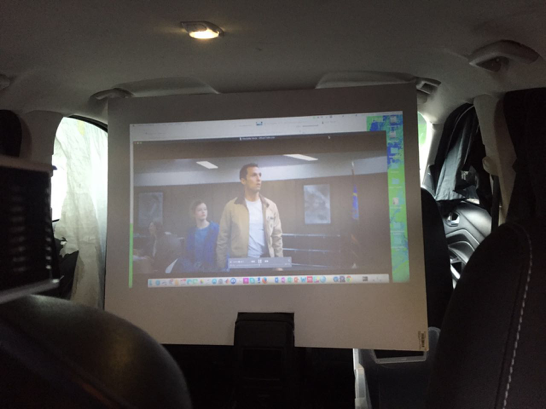
\includegraphics[width=5in]{Figures/Prototypes/DarkHorse/DarkHorseTheater1.png}
	\caption{In-car movie theater}
		\label{fig:DarkHorseTheater1}
\end{figure}

\begin{figure}
\centering
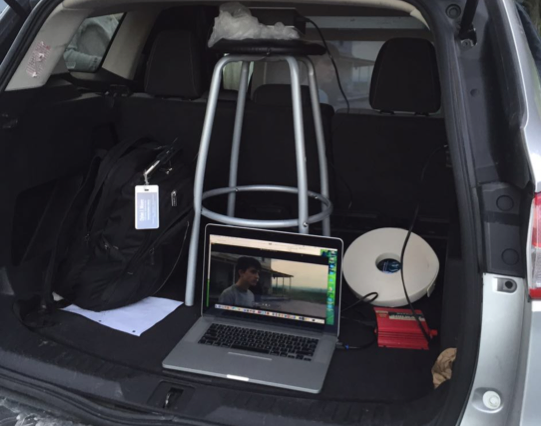
\includegraphics[width=5in]{Figures/Prototypes/DarkHorse/DarkHorseTheater2.png}
	\caption{In-car movie theater}
		\label{fig:DarkHorseTheater2}
\end{figure}

For the in-car meditation, we placed a diffused light shined beside the passenger, a sun-like warm light was also used. We also played New Age meditation music through car speakers.

\begin{figure}
\centering
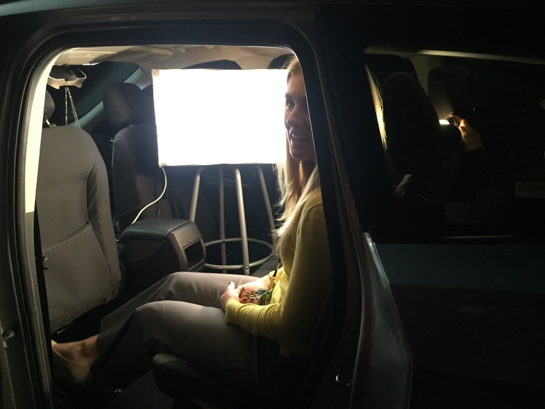
\includegraphics[width=5in]{Figures/Prototypes/DarkHorse/DarkHorseMeditation1.png}
	\caption{In-car meditation}
		\label{fig:DarkHorseMeditation1}
\end{figure}

\begin{figure}
\centering
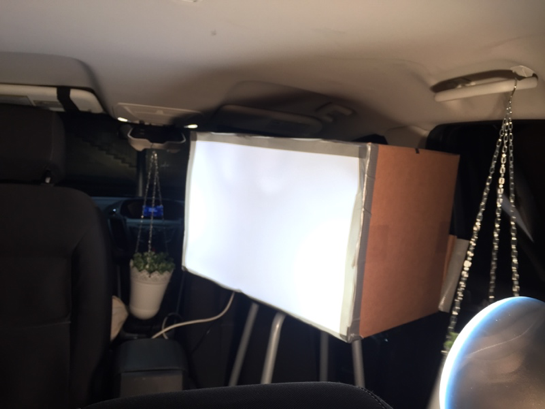
\includegraphics[width=5in]{Figures/Prototypes/DarkHorse/DarkHorseMeditation2.png}
	\caption{In-car meditation}
		\label{fig:DarkHorseMeditation2}
\end{figure}

We set up both prototypes in an SUV and tested them with some users. The insights we gained from interviews are:

\begin{itemize}
    \item Functional fixedness: Lots of people expected to watch the movie while driving, and were surprised when we said that it was for while the car was parked: people don't think of their car as an extended space while stationary - only think of it as moving from A to B. One driver mentioned that his car is associated with too much stress – commuting, work, etc. so he would not be able to relax in it.
    \item People were very comfortable and overall responded well to the experiences saying they were both fun and relaxing, but didn’t desire for them to be in their car. Some might pay a little extra while others would just want it in their home. Several expressed concern with setup time/hassle. 
    \item Several people said that they would like it if they had kids - the kids could watch a movie in the car while the parents had some peace and quiet in the home. Though the parents/families we talked to did not express much interest.
    \item One woman would go on a date in the movie theater as she liked the privacy.
    \item Power limitation - battery only lasted for 20-30 minutes of projection before it went low. We left the engine running for the meditation room. 
    \item Father with kids said he'd prefer it if he had an autonomous car and he could do it to/from work – his kids were with him and couldn’t sit still. Older man agreed he thought it would be useful for light therapy for people with SAD.

\end{itemize}

So going forward, there are three main takeaways: 1. The user test reiterates the need for simplicity in our final design – it can’t add any complexity to users’ lives; 2. There is a preconceived notion of the car as only transportation, which presents a potential opportunity if there was a compelling use case to develop it as a room when stationary. Cars are sophisticated machines that sit idle for much of their lives; 3. Cars are also a source of stress – how might we counteract the tendency for people to see cars as stressful experiences?


\subsection{FUNKtional System Prototype: Audi Scene}

For our FUNKtional System prototype, we want to solve two problems: (1) Smart home tech needs seamless integrated interfaces (set it and forget it) to manage technology and (2) Audi cars need to know users’ intention for departure to startup system (like an automated remote start). 

 Existing smart technologies are working on those problems: Amazon Echo is using voice control of home that connects to many devices; NuBryte home management system (out later 2016) sets lighting scenes for home, displays weather information, calendar, from a single source; Nimbus digital dashboard by Quirky displays simple information like “current time to home” and “tomorrow’s temperature”. The drawbacks with those devices are: More technological sophistication, but also more complexity. No dedicated physical interfaces. What if light switches changed their form depending on the day? It would get confusing.

Based on user needs, we image our solutions to be able to solve the problems in the approaches as shown in the following table.

\begin{center}
\tablefirsthead{%
\hline
\textbf{ } & \textbf{User needs to...} & \textbf{How might we address this need?} \\
\hline}
\tabletail{%
\hline
\multicolumn{3}{|l|}{\textit{\small{continued on next page}}}\\
\hline}
\tablelasttail{\hline}
\bottomcaption{From user need to approach}
\begin{supertabular}{| p{4mm} | p{60mm} | p{70mm} | }
		\hline 1 & Know his parents are safe. & He would feel better if his parents adopted smart home technology, but know it’s complicated. \\
		\hline 2 & Convince his parents to adopt smart home technology. & If he uses it and it’s simple to set up, then he can demonstrate to his parents and they will be more likely to use it.  \\ 
		\hline 3 & Control lighting, security, and temperature when he gets home to increase productivity. Wants control himself - doesn’t necessarily want home/car to “anticipate needs.”  & Placement of key fob triggers scenes in home, eliminating need to turn on/off lights, lock door, set music, etc.  \\ 
		\hline  4 & Boot Audi infotainment system before he gets to car to establish connection to internet. & Removal of key fob sends indication to car to begin 1 minute process. Could also set climate control. \\ 
        \hline 5 & Turn off lights, adjust heat, and make sure door is locked before he leaves home & Removal of key fob triggers “leaving home scene” that make sure no energy is being wasted and home is secure before he leaves. \\
        \hline 6 & Manage different media sources in his home. & Transfer media from car, start media when user arrives home if preprogrammed under scene. \\
\end{supertabular}
\end{center}

We designed a key fob storage unit that sets initial state of smart home when key fob is dropped into bin and signals car and home that user is leaving as key fob is picked up. As you walk in your front door, you can put your key fob into one of four bins that triggers a different “scene” for your home. E.g. relaxation mode turns on softer lights and nice music and work mode turns on brighter lights; It also continues media from car to home (e.g. sports match on radio to TV). It is customizable, and will eventually give smart suggestions. When leaving home, removal of key fob sends signal to car that starts up infotainment system (current time is appx. 1 minute) to connect to internet (e.g. pull addresses/traffic from Google Maps), and sets climate control. It also tells smart door lock to lock behind you (better than walking away and assuming door will lock behind you). 

\begin{figure}
\centering
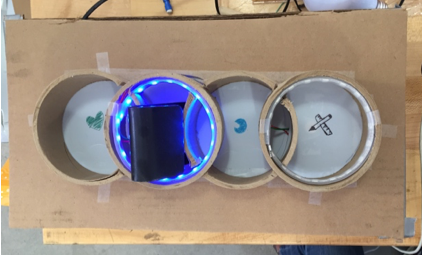
\includegraphics[width=5in]{Figures/Prototypes/Funky/FunkyPrototype.png}
	\caption{Drop the key fob to set different scenes for your home.}
		\label{fig:FunkyPrototype}
\end{figure}

\begin{figure}
\centering
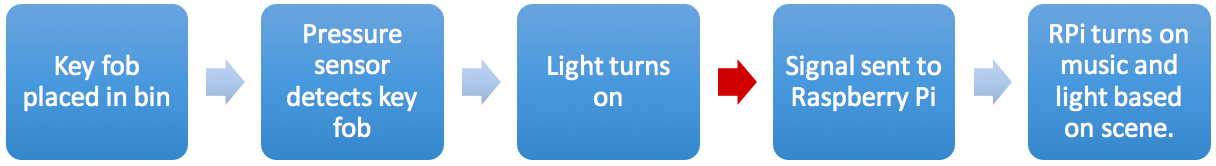
\includegraphics[width=5in]{Figures/Prototypes/Funky/FunkyPrototypePrinciple.png}
	\caption{Description of system working principle}
		\label{fig:FunkyPrototypePrinciple}
\end{figure}

From building this prototype, we have learned (1) online webserver and scripting is very powerful - we can leave many control function running on web server instead of portable hardware; (2) Lutron smart switch used different communication protocol and is not disclosed to customers, it is difficult to match them even for developers. But we were able to buy more generic ones; (3) However the simple physical operation is easy to use and could probably be adopted by even the most technologically compromised users.

And for future development, we have discussed the following potential features:

\begin{itemize}
\item Light string can display state of home through colors as user approaches to retrieve fob.
    \subitem Red: something needs to be addressed (e.g. door or window open)
    \subitem Yellow: almost ready to go, and system can take care of it (e.g. light on)
    \subitem Green: all set to walk out the door (all lights off, etc.)
\item RFID tags for important items detected by system - intelligent state selection (e.g. if briefcase is detected, then car will know user is heading to work). Also could alert user if something is forgotten at home or if something is left in car.
\item Address security desire in smart home –incorporate a monitoring element (e.g. if a package is delivered, door can open and system can record delivery to make sure nothing is stolen).
\item Wireless charging of key fob while it is in the device.
\end{itemize}
\section{AudiDefender}
\subsection{Description}
% Shouldn't we leave the distinction between HPI and Stanford out?
"Audi Defender" is the most complete prototype that reflects our vision with regards to security. According to design requirements, the system should securely detect the keyfob and verify its identity, and then enabling quick arming and disarming of home security system. The system should also interact with users and provide instant feedback about car and home, presumably but not limited to a visual display. Along with Stanford's Funky prototype, we designed a bin that would be placed in people's home to represent Audi's brand. The system wirelessly connected to a touchscreen that displays security status of home and car as well as car's driving range. These information are deemed crucial in the transition space of car and home. 

We think the security angle is appropriate for Audi to tackle with in this joint realm of home and car. Firstly, people have trust in car's security system, and Audi have sophisticated related technology that can be relatively easily used in this system. Secondly, leveraging existing car security system could make interface simple and reduce the need for another isolated security token. Finally, it is the security related information that people mostly want to know about their car while they stays at home. And the (visual) interface of such a device can well serve that purpose.

In summary, our system is a physical presence of the car in your home. Presumably, it is placed on the table and looks cool like other Audi accessories [\url http://audicollectionusa.com/Accessories]. It works with user's keyfob to smooth the secure transition from home to car and provide valuable security status to user to let them feel carefree about their home and car. A video of how we imagine this system improving users' lives can be found here \url{https://youtu.be/NIcLD-aaaGM}.

\subsection{Implementation}
\begin{figure}[ht]
\label{Fig.AudiDefender}
\centering
	\includegraphics[keepaspectratio, width=5in]{Figures/Specifications/AudiDefender.JPG}
	\caption{Stanford's Prototype, a electronics device to put on a table inside the home. Its touchscreen shows car and home related critical information, and it interacts with a special Audi keyfob to arm and disarm smart home security system. At the top of it there is a bin to store and verify user's Audi keyfob}
\end{figure}

As depicted in Fig. \ref{Fig.AudiDefender}, this prototype is designed to be placed on a table in the home, possibly near the front door. It is primarily made of black foam board. At the front side, there is a touchscreen to provide visual interactive interface to the user. It also plays alert sounds in emergency. At the top of the device there is a bin to place the keyfob, and user need to interact with our system using our special Audi keyfob. Electronics is placed inside the box and a large battery bank support the mobile use of electronics. The touchscreen shows security status of the home and car, whose state transition is illustrated in Fig. \ref{Fig.StateChange}

\begin{figure}[ht]
\label{Fig.StateChange}
\centering
	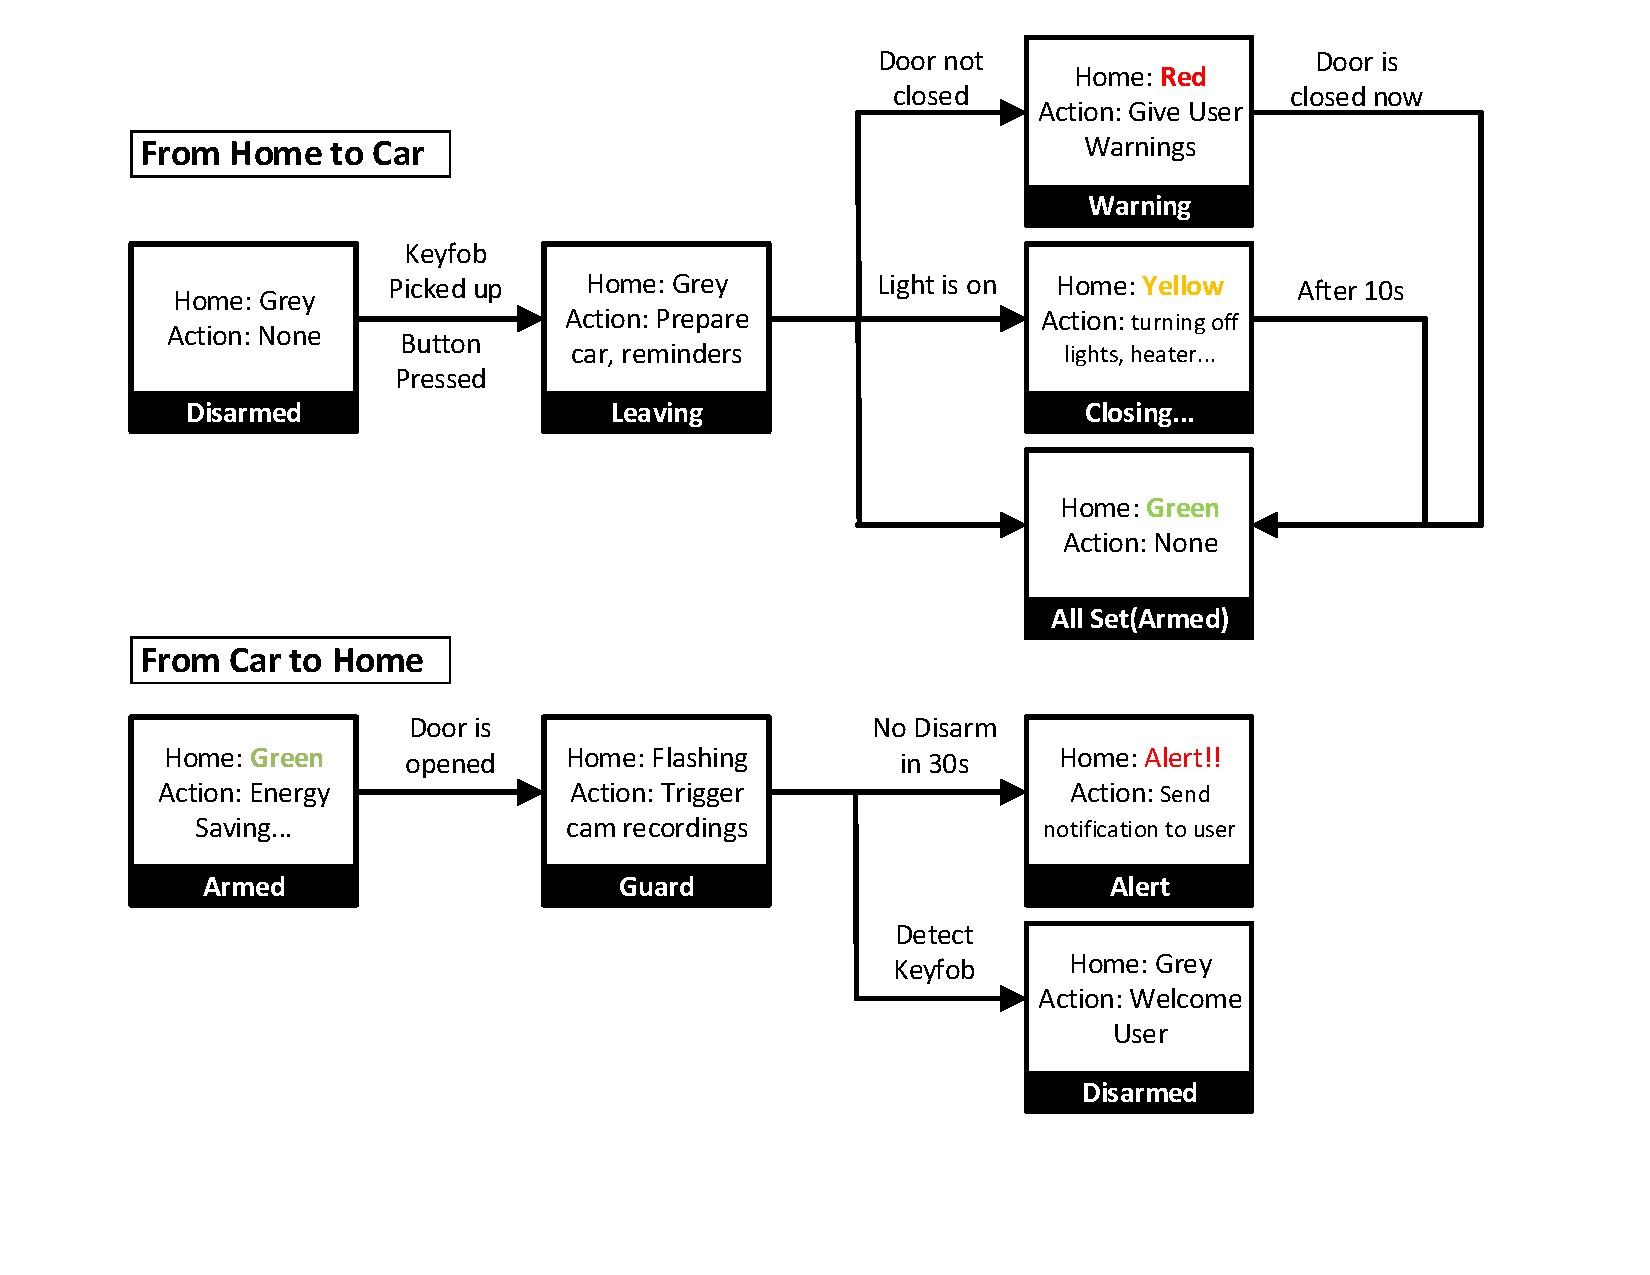
\includegraphics[keepaspectratio, width=5in]{Figures/Specifications/StateDiagram.pdf}
	\caption{State transition diagram for both case for going into home and leaving home. It described which color to display for the home icon in that touchscreen. In a certain state, there are smart home activities and settings associated with the status.}
\end{figure}

The bin provides a place to store the keyfob, and we check the keyfob using RFID(Radio Frequency Identification) chips and reader. RFID is a short range communication method, so it avoids the hackability of long-range radio signals. However, we used only a "passive" card in the keyfob, which code can be read by any other RFID reader. Going forward, we definitely need to use a more sophisticated secure communication method and advanced techniques like rolling codes. Accordingly, we should consider factors like the battery life of the keyfob, and sophisticated protocol. Henceforth in our prototype, in order to avoid complexity in prototyping, only simple RFID communication is used. A 125kHz RFID card is placed into the shell of a Audi keyfob to create our special keyfob, and a card reader kit is placed inside the bin. When the special keyfob is moved towards the reader, the reader gives off a beep sound and send the unique identification code of card via serial port. By matching the signal with recorded code in system, the controller unlocks the security system.

We used Raspberry Pi 2(RPi) as our central controller. It runs a LINUX based operation system, and can thus achieve versatile functions. RPi has more memory resources and available open library than microcontrollers like Arduino, but it has drawbacks in handling real-time tasks. We used python for most of the programming and vncserver and SSH to communicate with the RPi in Wifi netword during programming and debugging.

\begin{figure}[ht]
\label{Fig.AndroidInterface}
\centering
	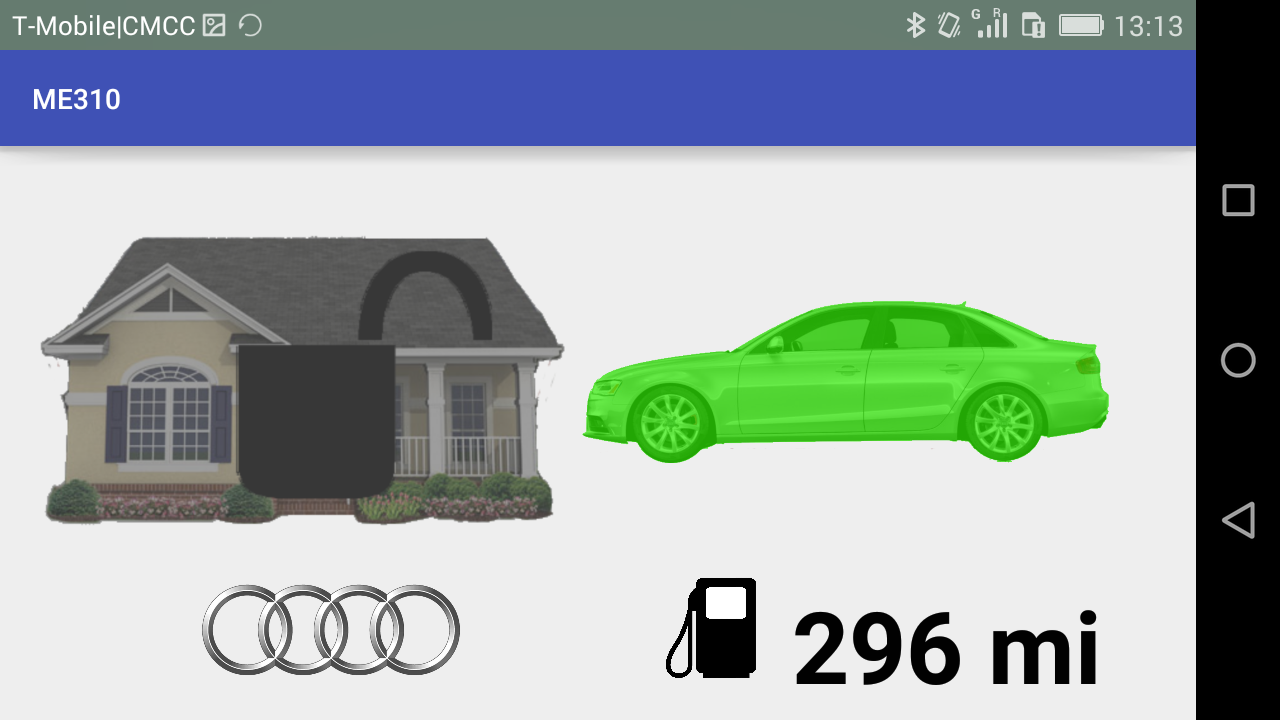
\includegraphics[keepaspectratio, width=5in]{Figures/Specifications/AndriodApp.png}
	\caption{Enlarged touch screen, enabled by a Android App. It has simple intuitive state indication, and after user pressed the icon, detailed information would be prompted}
\end{figure}

The touchscreen display in our prototype is a Huawei smartphone running android system. The android interface is designed as showed in Fig.\ref{Fig.AndroidInterface} The icon of car and home associated with different colors shows the security status as fully explained in Fig. \ref{Fig.Icons} . After the user long pressed the icon, detailed text notification will be prompted. In our prototype, we lacks input from car, so we made the car icon color changing for long-press to facilitate demo.

\begin{figure}[ht]
\label{Fig.Icons}
\centering
	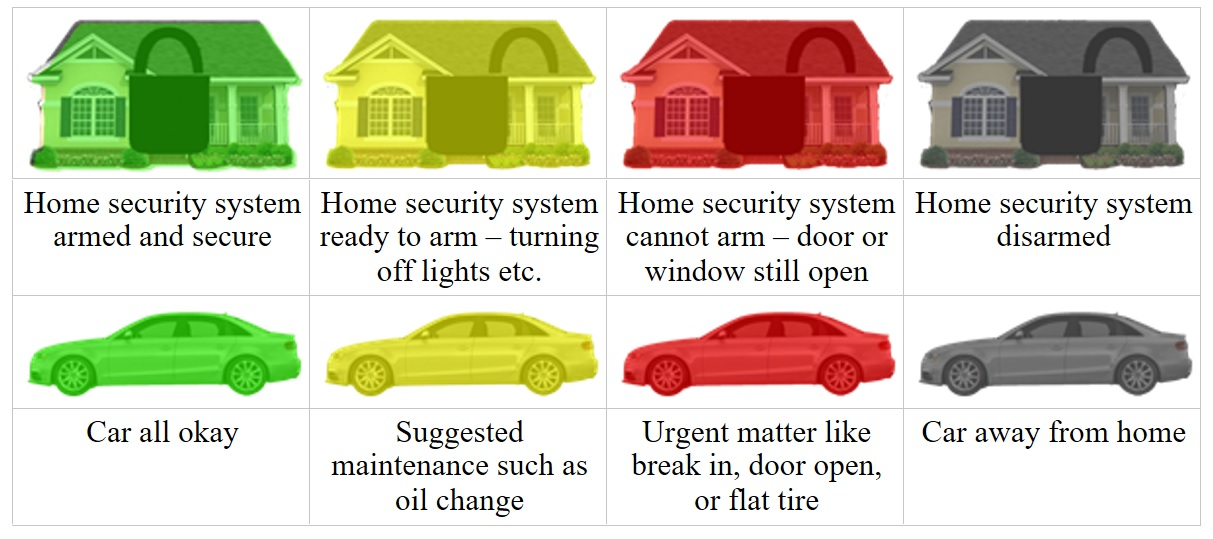
\includegraphics[keepaspectratio, width=5in]{Figures/Specifications/Icons.jpg}
	\caption{Different icons and explanation for the interactive touchscreen. Notice that we only implemented the automatic change of home's icon in the prototype. We still lack car side's input.}
\end{figure}

For simplicity, we used Bluetooth to communicate between RPi and smartphone. A serial port is established via Bluetooth, and the Rpi send code in the format of "H[State]\#[Information]" ([State] is a number from 1 to 4, and [Information] is a string)to control the displayed home status. Since in our system we cannot automatically detect the leave of keyfob, we need a switch to tell the system the change of state. We implemented via the smartphone, when the home system is disarmed and user pressed the home icon, a message of "LEAVING\#"is sent to RPi and it will change system status accordingly.

There are many tasks for the systems to handle during the Leaving state. Actually it is a requirement for the system to reliably detect user's intention of going to the car. If the ecosystem obtained that intention to car in advance, it can boot the infotainment system to avoid long reboot time and preheat the car. The ecosystem can also present mobility related information and reminder to prepare the trip like we did in our CEP. However, in our prototype, we temporarily saved these aspects for future development and focus on the smart home aspect as expalined in \ref{Fig.StateChange}. After the user dictate their intention to leave, the system check the status of home. If some major door or window is still open, the system display red home icon and require user to fix that. If some lights is still on, the system display yellow icon and it means some issues is automatically taken care of by the smart home and icon quickly changes into green meaning you are free to leave. By providing simple visual feedback, user will have overview and control of their home and they can always look into details.

Initially, the system is built upon scratches from related open-source RPi  projects. The most extensive one of them is "PrivateEyePi" [http://projects.privateeyepi.com/], which is the foundation of some early developments. For debugging, we built a system  that connects LEDs, buttons, LCD to Rpi. But we later abandoned those and transferred most of the interface to the touchscreen. We have also attached buzzer to RPi, but for final prototype, we used sounds of the smartphone instead to simplify the hardware. 

According to the system diagram, the system should connect to existing smart home to get necessary input about the status of the home. Due to the complexity of commercial system, especially the communication part, we must simplify this part to certain extent. Firstly, we have built a small scale home paper model that use contact switch (relay) to detect the status of the window and doors as showed in Fig. \ref{Fig.SmallHome}. This modelling resembles the actual home security sensor quite much, but we found this model is difficult for user testing and smart home system is an unnecessary complexity in our prototype.

\begin{figure}[ht]
\label{Fig.SmallHome}
\centering
	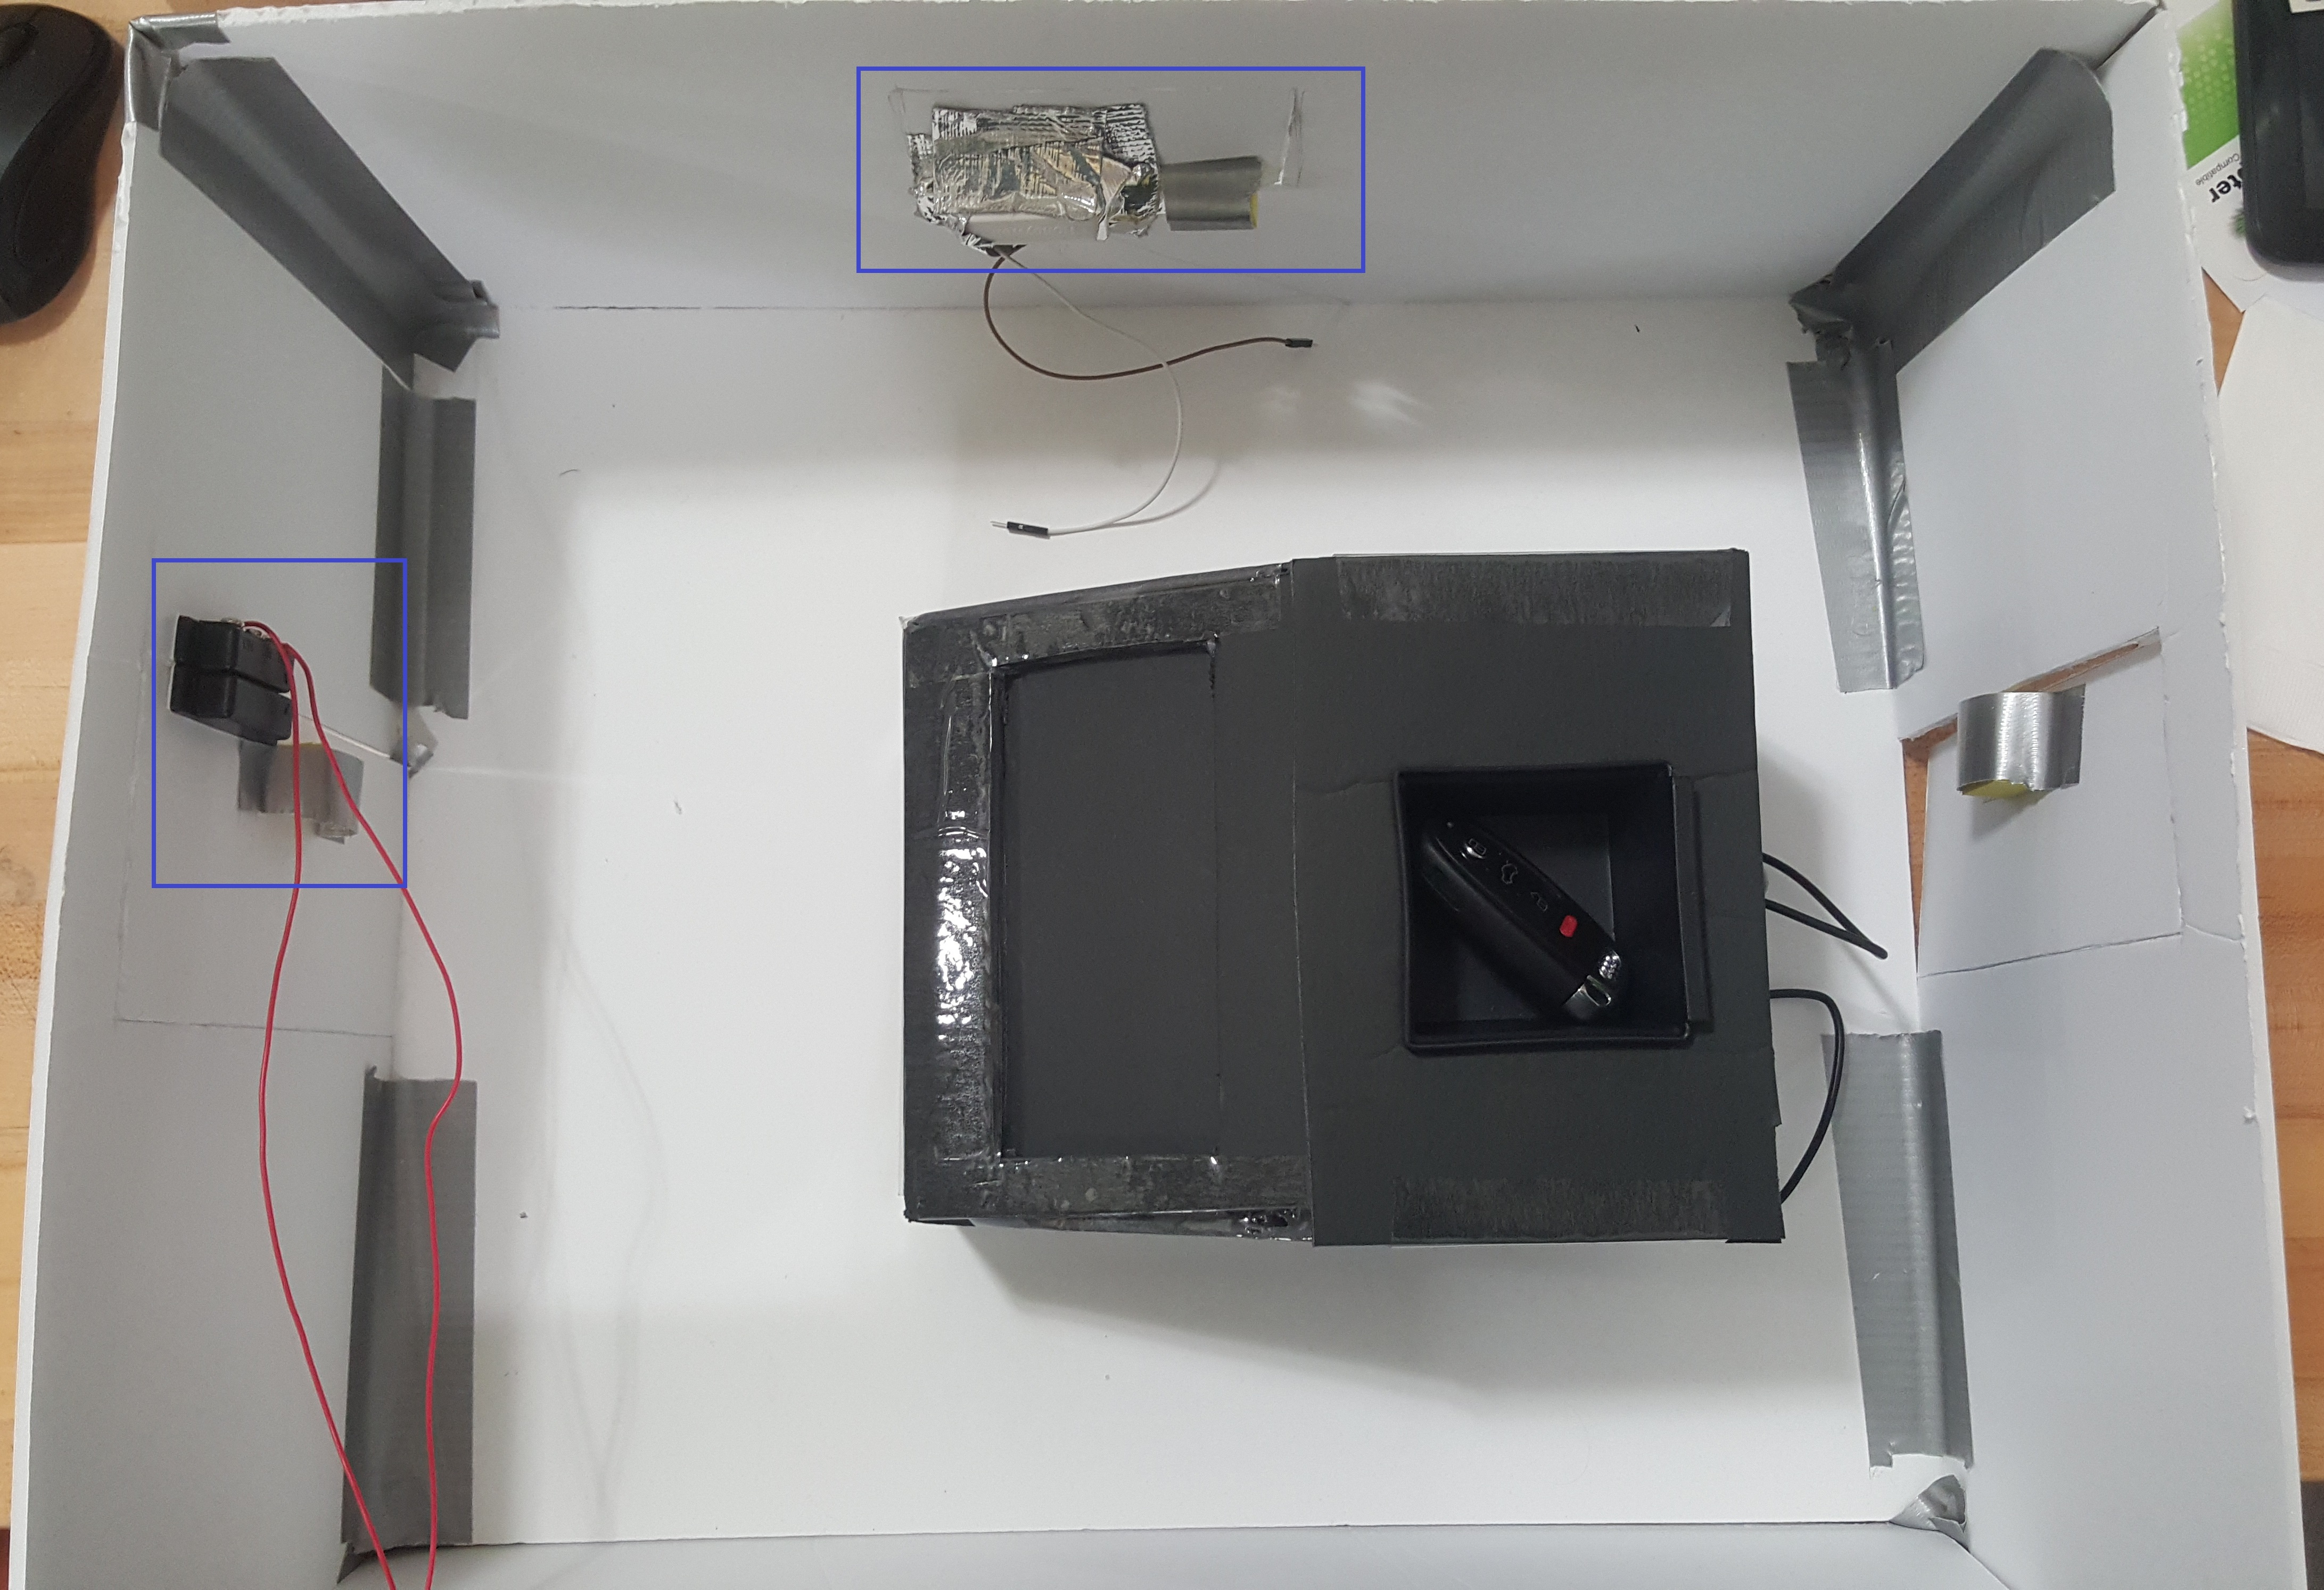
\includegraphics[keepaspectratio, width=5in]{Figures/Specifications/SmallHome.jpg}
	\caption{A small scale home model build from cardboard. Blue rectangle illustrates the contact sensor that indicate the on/off status of windows and doors. }
\end{figure}

\begin{figure}[ht]
\label{Fig.VirtualInput}
\centering
	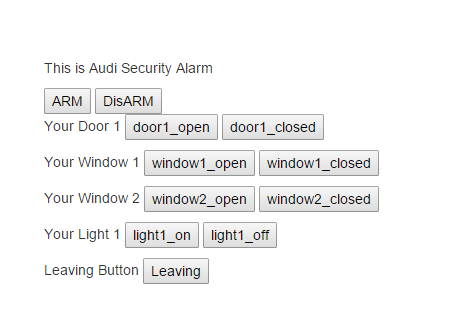
\includegraphics[keepaspectratio, width=5in]{Figures/Specifications/VirtualInput.png}
	\caption{A virtual version of the smart home architecture. By pressing the button on the webpage, we give system input about home status, thus eliminating the need to implementing smart home hardware in our prototype. In our vision, we assume this Audi prototype will not change the basic smart home architecture, but to communicate with its controller}
\end{figure}

Later, we adopted a simulation method to get virtual smart home input from a webpage. The picture Fig. \ref{Fig.VirtualInput} shows that we can directly dictate status of window, door and lights. It also has buttons to directly change the state to facilitate debugging. In order to create webpage, we firstly used a python module called "WebPy" and later transformed to "Flask" combined with simple HTML. These newly developed tool is quick to use, but due to our inexperience in front-end programming and Linux, we only implemented basic interfaces and logic. The use of webpage also arise the use of multiprocessing, since RPi needs to process webpage response, communication, state transition based on home input simultaneously. Basic python multiprocessing module is used and need further explored to address some unreliability in existing system.

We have performed several technical tests throughout the development and we can see that communication protocol and growing complexity is a challenge. We improved the structure of the device to make it fit for electronics and battery, better looking, screen tilted for easy touch and display. We primarily tested at the entrance of Stanford bookstore. And at the parent's day, it appeared lots of parents have Audi cars and many of them has experience with security system, which makes them good representatives of our persona. They generally respond excited to our prototype. The physical presence of the car in home itself seems innovative to them too.  Many users told that this device would reinforce the habit to put keyfob in a certain place, and many of them likes to do so to restrain from forgetting the keychains. …

\section{AudiSeamless}

AudiSeamless is a system that wants to make forgetting things a thing of the past, at least with respect to what a user needs to take care of before leaving the house. It contains all of the findings of previous prototypes\footnote{described in the appendix under \ref{sec:HPIPrototypes}} but goes more in the vain of providing a system that is of use at home, as opposed to the earlier prototypes which were more useful on the road.

During interviews, we found out that there are three areas that people need to be assured about before being able to leave their homes with an easy mind:

\begin{enumerate}
    \item House: This includes making sure the heating is turned off, that all windows are closed and that the home security system is armed.
    \item Packing: Users have to be sure that they packed everything they will need like luggage before a longer journey or their sports items for their training.
    \item Car: This includes knowing where the car is parked (a challenge in big cities, especially when sharing the car with family members), whether the car's windows are frozen and how much gas is left in the tank.
\end{enumerate}

\noindent{}AudiSeamless collects information for every connected device in these three areas and makes this information available to output devices like smart phones, voice assistants like Amazon Echo or our corresponding idea, \textbf{AudiBits} (see Figure \ref{fig:AudiSeamless}). The intended use case for AudiSeamless is to provide the necessary information at the right time and place for users so they forget things less often. So when a user is about to leave their house, AudiSeamless is supposed to indicate to her that she forgot to pack her sports bag for the night.

AudiBits (see Figure \ref{fig:AudiBits}) are specifically tailored to this use case: They are small, single-purpose displays that show information about one specific item. They can be placed in any part of a user's home to maximize usefulness to them. So if the user had connected her AudiBit with her sports bag and placed it near her house door, she would recognize that she had forgotten it before leaving the house, thus saving her time.

\begin{figure}[ht]
\centering
	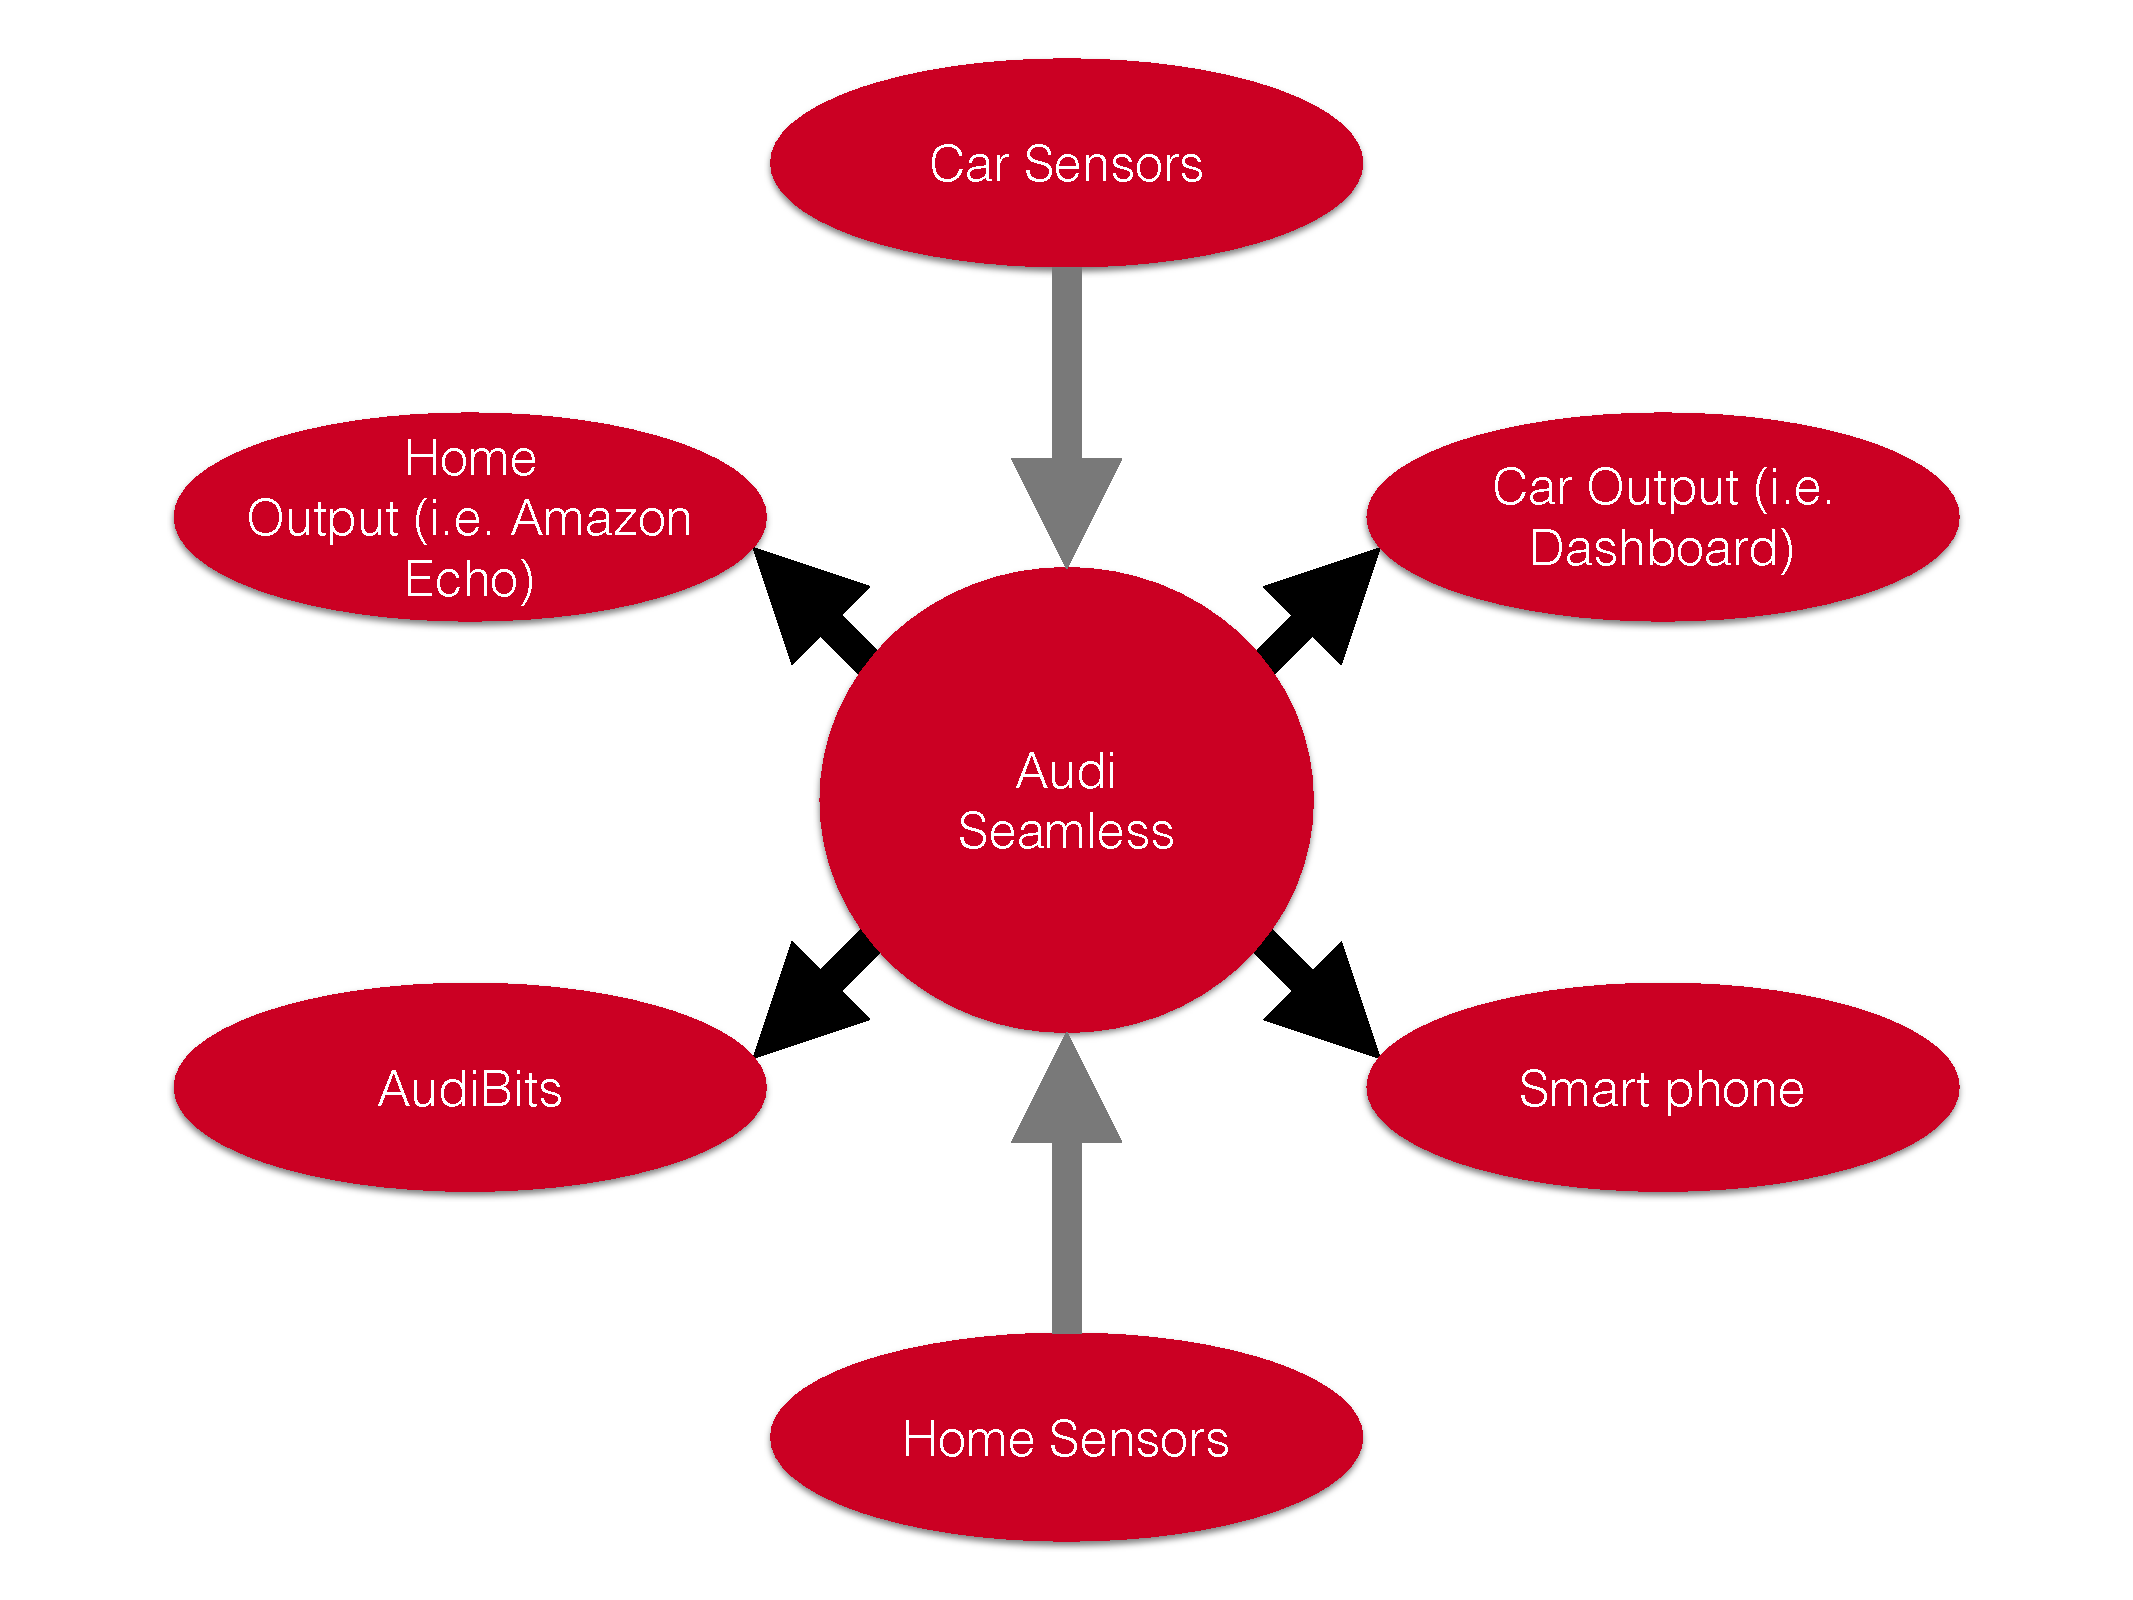
\includegraphics[keepaspectratio, width=\textwidth]{Figures/Specifications/AudiSeamless}
	\caption{The AudiSeamless concept works with home and car data sources and distributes the collected data to different output devices like smart phones.}
	\label{fig:AudiSeamless}
\end{figure}

\begin{figure}[ht]
\centering
	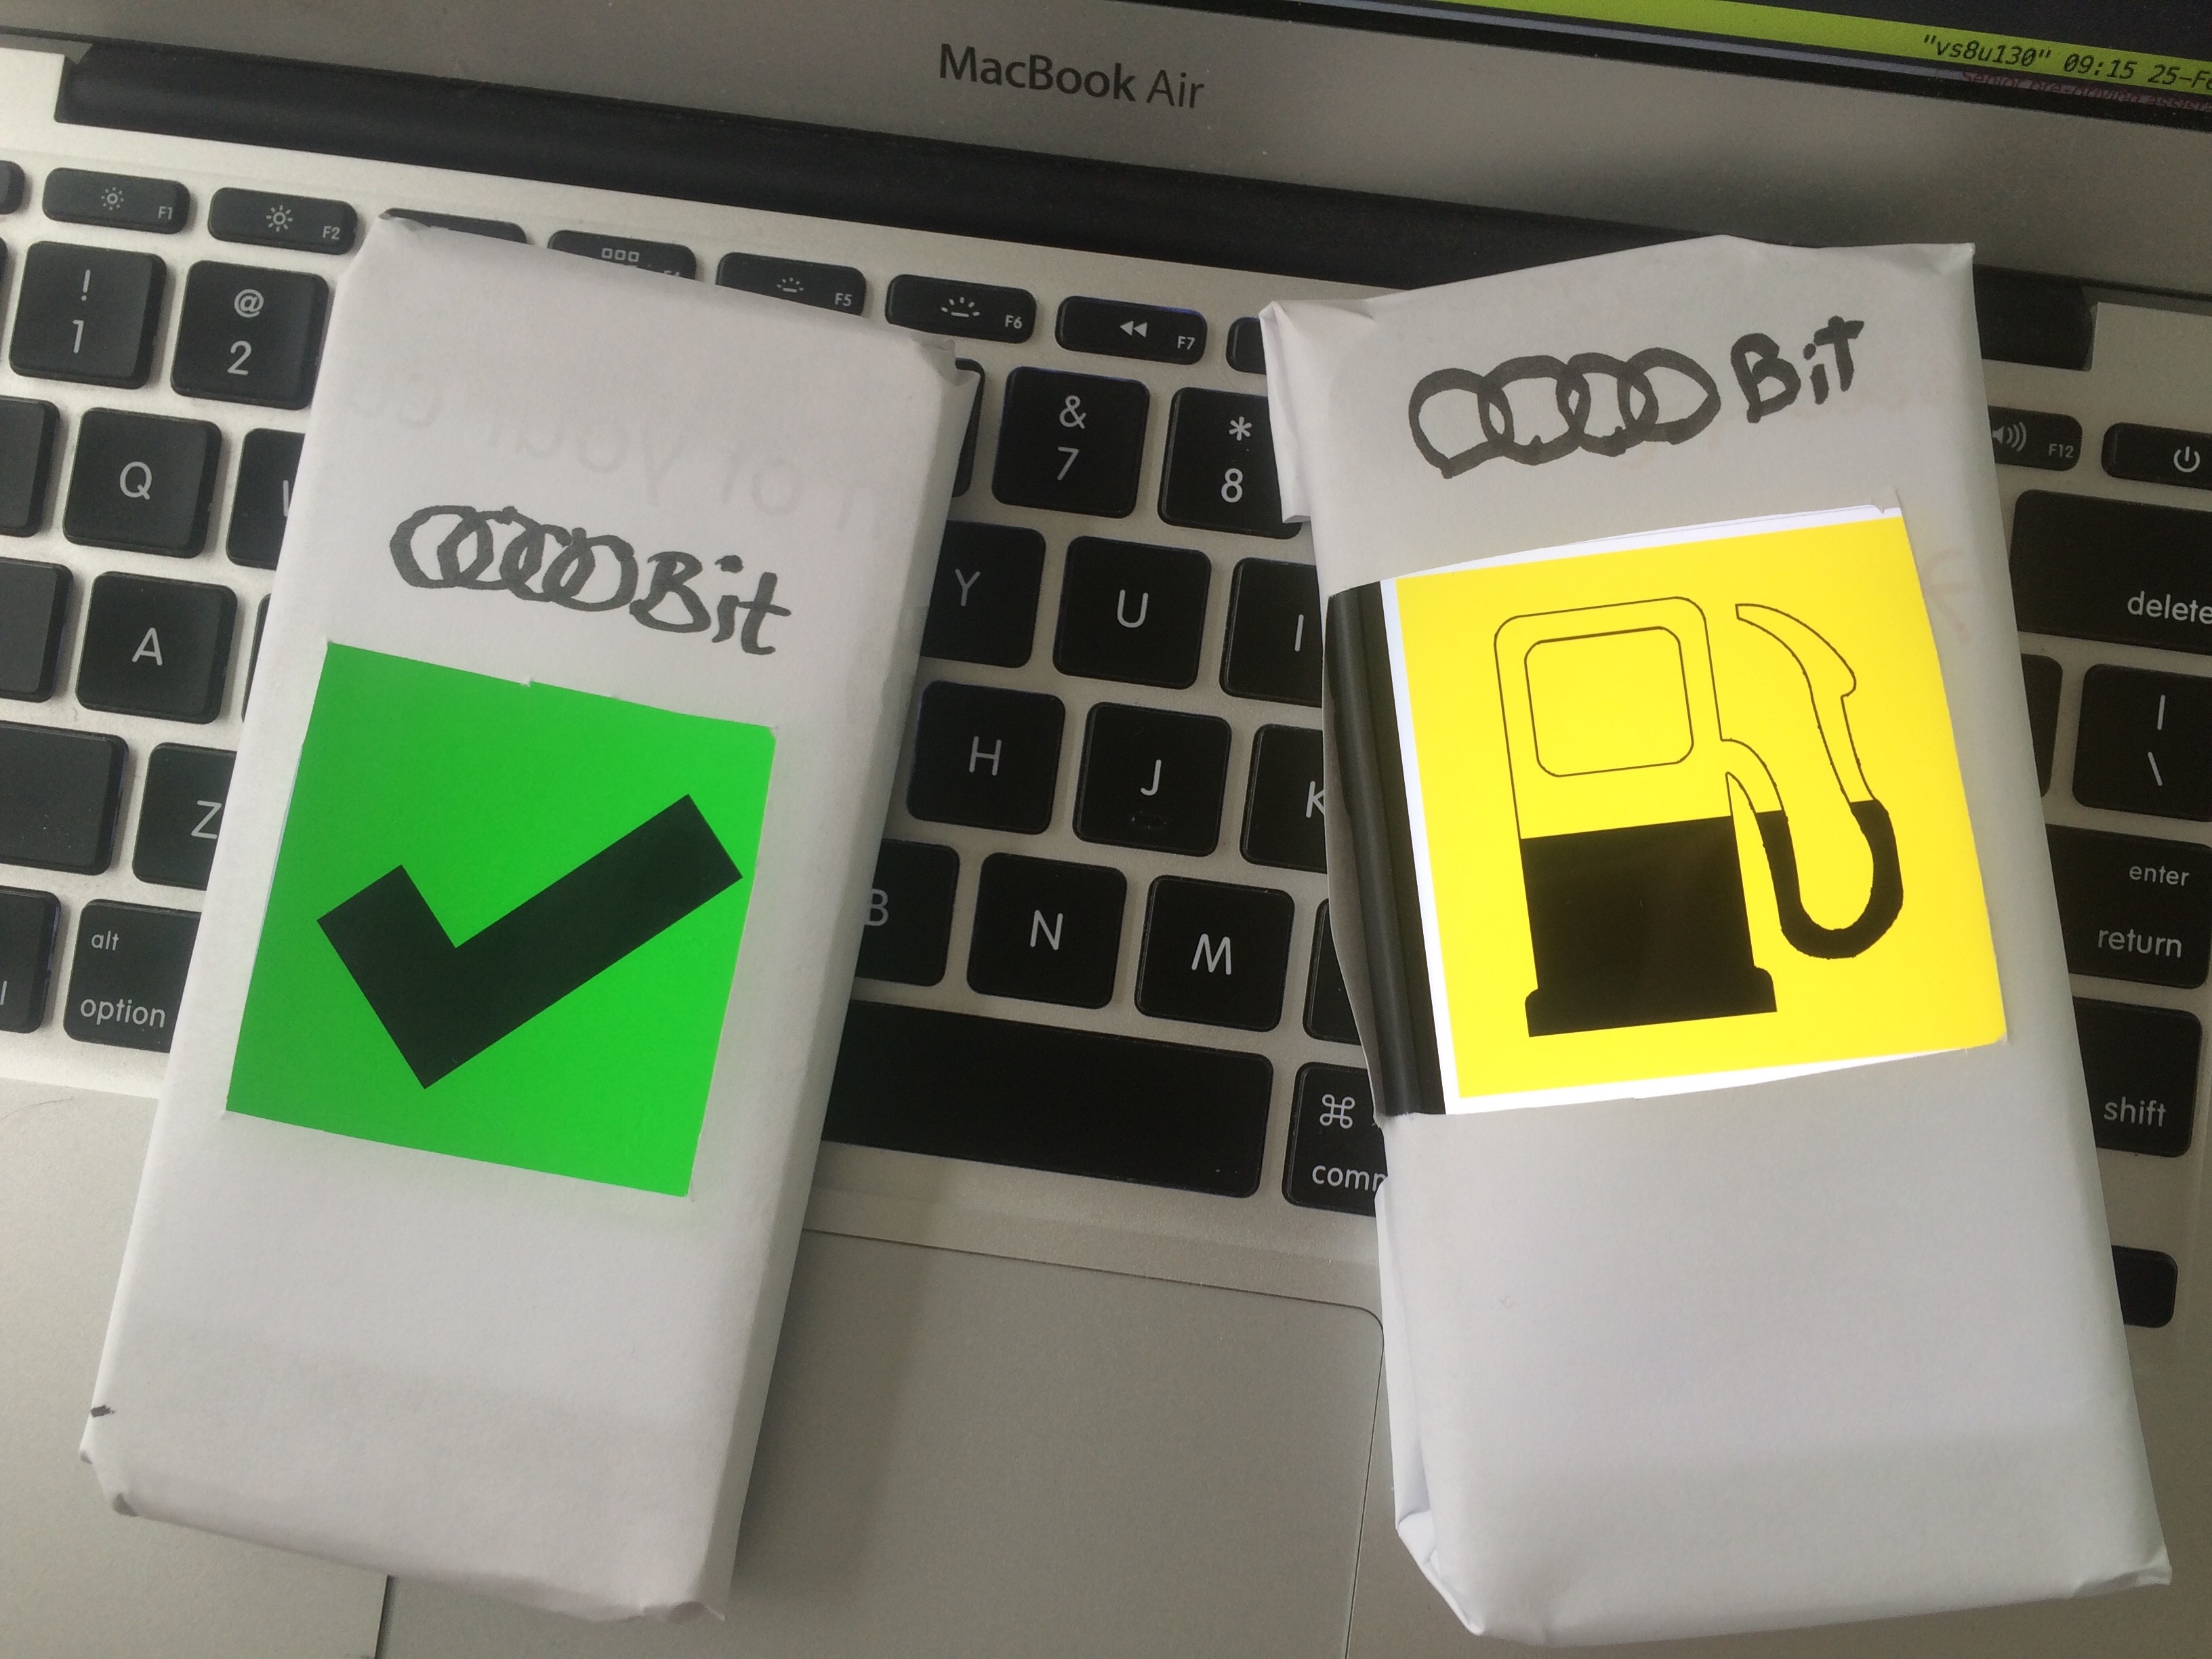
\includegraphics[keepaspectratio, width=\textwidth]{Figures/Specifications/AudiBits}
	\caption{Two AudiBits. The one on the left shows an item that has been taken care of and the one on the right shows the gas tank, both with an icon and with a color (green = tank is (almost) full, yellow = tank is about halfway filled, red = tank is (almost) empty)}
	\label{fig:AudiBits}
\end{figure}

The AudiBits purposely represent a semi-automatic approach to keeping an eye on the users homes and cars. Many use cases of AudiSeamless seem like they could also be completely automated. Instead of reminding the user or displaying information to him the system could act itself without interacting with the user, one could think. Instead, we have identified that our users want to have the feeling of being in control, to have the last word. The AudiBits build on these findings by displaying bits of information to the user and letting her interact with them when she wants to. They stay unobtrusively in the background if she decides to ignore them.

We tested this idea with potential users and received positive feedback to the idea itself and the underlying need but also heard from many people that they don't see the need for small displays like the AudiBits since their smart phones can also display the same data. We agree that this is possible but still find that AudiBits offer a significant improvement: They are always visible at places where users will see them when necessary as opposed to a smart phone with which users have to first open up an app or take them out to look at a notification and which are not always with the user.

We also found out that merely displaying the status of a forgotten thing is not enough for users because they want to be able to act upon it. For example, if the display shows that the user's car windows are frozen, he wants to be able to turn on the heating so that he can start driving as soon as he reaches the car without having to get rid of the ice on the car windows first.

Another finding is that people think of things they need to do when they're home while they're out. AudiSeamless and especially AudiBits could be a good way of resolving this: While out, the user could send whatever they want to remember to AudiSeamless which an AudiBit set up for this purpose could then display so the user sees it when they get back home.

\clearpage


\section{User Journey}
Our persona Linda has to get up very early in the morning, and really is not a morning person, so she's often still groggy when she leaves. As a result, she forgets to bring sports equipment for days when she exercises, or an umbrella when it's going to rain that day. AudiSeamless will remind Linda that Tuesdays and Thursdays are her CrossFit days and that she should bring her gym bag if she does not already have it. As a result, less of her classes will be skipped due to not having the right equipment.

When Linda gets home from a busy day at work, and then CrossFit, and nobody else is home, the last thing she wants to do is worry about forgetting to disarm her security system, have the alarm go off, and have to pay a fine for a false alarm. However, she does like the peace of mind that her home is being looked after during the day, as there have been a couple of break-ins in her neighborhood recently. She also likes to know that the home will be secure when her kids get home from school, and that they can each disarm the system with a mini Audi key fob on their keychains. Her daughters love showing off the key fobs at school.

Using AudiSeamless, she gets peace of mind of the home security system while not changing her daily routine at all. She often keeps her keys in her purse, so when she walks in the door, the key fob's presence is automatically detected and the home security system  automatically deactivates. She might even want to set up a light or two to go on at that time, so that she can easily find her way through her front hallway. 

However her family members like to store their keys, either in a bag or in their pockets, the system can detect their presence and store their keychains if desired (see Figure \ref{fig:Vision}). The system also interacts with modular displays that show basic information about her home and car. She can make sure her car is okay when she's inside her home.

\begin{figure}[ht]
\centering
	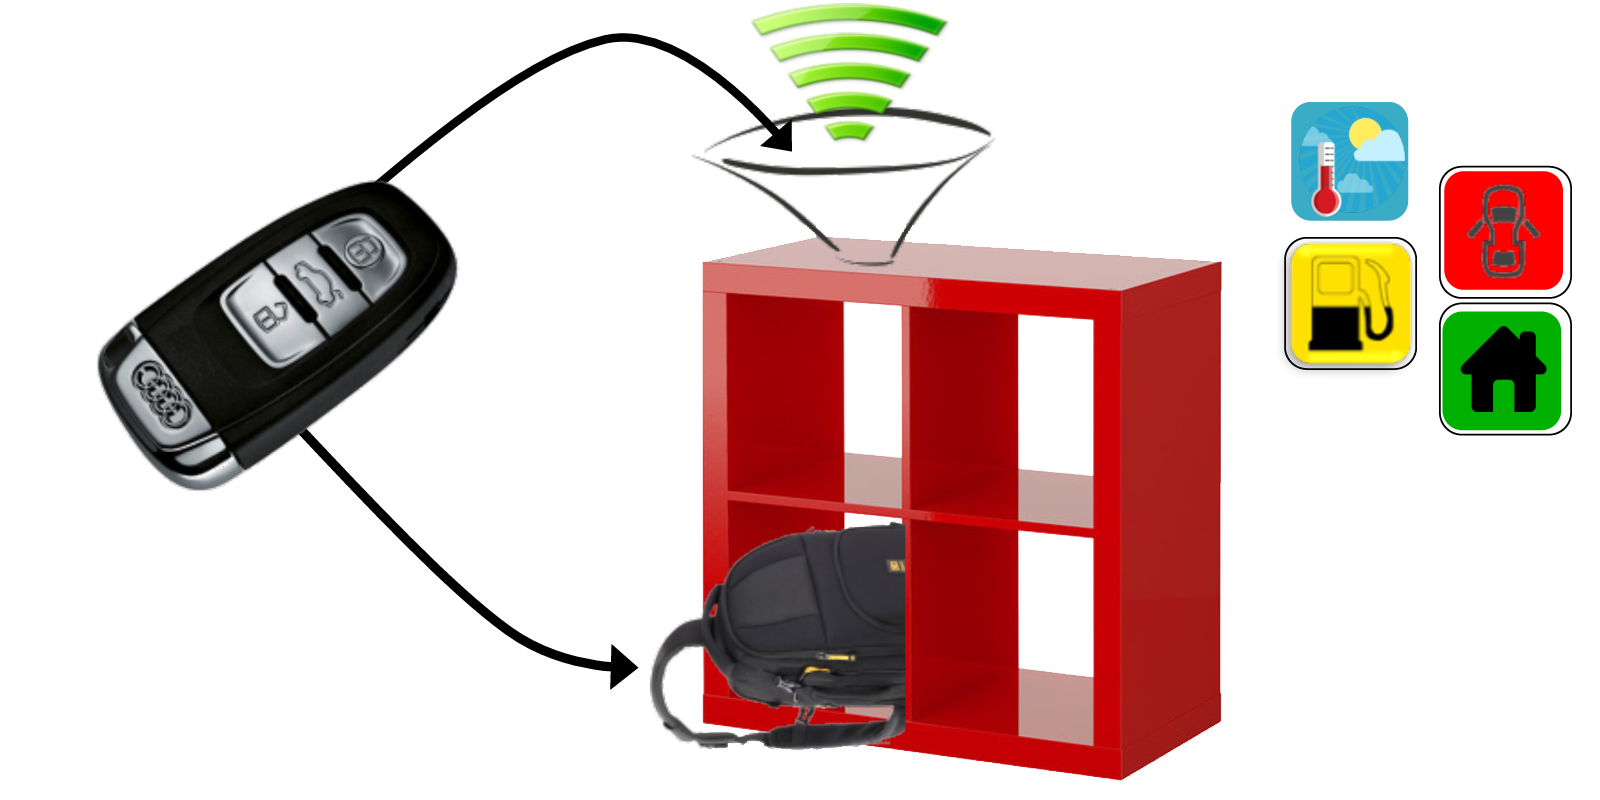
\includegraphics[keepaspectratio, width=6in]{Figures/Specifications/vision.jpg}
	\caption[Design vision overview]{An elegant bowl that wirelessly detects the presence of the Audi key fob to automatically disarm a home security system when the user arrives home. The bowl works in tandem with a set of modular displays that show important information about the state of the home and car and placed anywhere the user desires. Upon departure, the user’s indication of departure prepares their Audi for the journey ahead by setting car’s climate, heating electric batteries, connecting car to internet, and reminding them of their parked car location.}
	\label{fig:Vision}
	
\end{figure}

\section{Ongoing Development}

There are some remaining questions we are currently investigating.

\begin{itemize}
    \item How should the system interact with multiple key fobs in use with access to the home security system and car?
    \item What is the ideal placement for the display or whatever visual feedback users receive about the state of their car and home? Should it be integrated with the system or modular to be able to be placed anywhere?
    \item What is the best way to communicate home and car-related information? We will test interfaces including, but not limited to, lights, audio, visuals, all through a display, smart phone, and/or the key fob itself.
\end{itemize}
    
\noindent There are also many technical improvements to be done. We need a seamless integration of the physical device and electronics and we will let the user interact with our prototype rather than showing its function by ourselves. The main challenge would be communication, reliable state change, and interaction design. However, due to the tight security of the Audi key fob system and multimedia interface, for obvious reasons, we will have to simulate the key fob communication and car communication using other protocols, so we can spend more of our effort on fine-tuning the experience we want to give our users.